\documentclass{article}
\usepackage{fullpage}
\renewcommand{\familydefault}{\sfdefault}
\usepackage[scaled=1]{helvet}
\usepackage[helvet]{sfmath}
\usepackage{graphicx,amssymb}
\everymath={\sf}

\usepackage{parskip}
\usepackage[colorinlistoftodos]{todonotes}
\usepackage[colorlinks=true, allcolors=blue]{hyperref}
\usepackage{multicol}
\usepackage{float}
\newcommand{\TeaserImage}[1]{\raisebox{%
  .5\dimexpr-\height+\ht\strutbox-\dp\strutbox}{%
  \includegraphics[width=0.29\textwidth]{#1}}}
\title{Stethoscope Mold Making SOP}
\author{Gyan Edbert Zesiro}
%\company{The University of Western Ontario}
\setcounter{tocdepth}{2}
\begin{document}
\date{June 15, 2024}
\maketitle
\tableofcontents
\newpage

\section{Introduction} 
This document explains the process and safety procedure for mold making. We will go through how the materials and apparatus needed for mold making, testing the mold, and lab safety.

Since SimPL doesn't have the necessary equipment to do mold making, we are using \href{https://www.ampel.ubc.ca/facilities/shared-soft-lithography-facility/}{AMPEL 143A} lab space to make mold instead. 
Beware that AMPEL 143A does have a lot of dangerous chemical, so safety precautions must be taken, see \href{https://www.ampel.ubc.ca/safety-2/}{AMPEL Safety} for more detail. 

\subsection{Chemical Safety}
If you are using AMPEL lab space, chances are you need \href{http://rms.ubc.ca/training-and-general-education-courses/research-safety-training-courses/chemical-safety-training/}{chemical safety training}.This training takes a fair amount of time, as you need to schedule for a practical exam which might be booked for a long time. So best advice is to get this training done as soon as possible.

\section{Procedure}
\subsection{Material and Apparatus}
Here are the list of materials you need.
\begin{enumerate}
    \item Silicone casting material:\\
        Usually we will be using platinum-cured silicone, as they are contact safe and cure pretty quickly. You need to find silicone that best suit your need. Chances are, you will be buying your material from \href{https://www.smooth-on.com/}{Smooth-On}, a company specializing in mold making.
    \item Mold: \\
        A mold for your silicone polymer to cure. You can design a mold on your choice of CAD software and print them. Just make sure to have mold design in mind. Things to keep track when designing this mold are:
    \item Plastic or Paper Cup
    \item Popsicle stick
    \item Non-stick spray
        \begin{itemize}
            \item How to create the desired shape in mind
            \item How to prevent silicone from spilling
            \item Where do I pour my silicone
            \item How do I extract my cured mold
        \end{itemize}
\end{enumerate}
Here are the list of equipment you will need, note that someone will need to train you on how to use these equipments.
\begin{enumerate}
    \item Centrifugal mixer
    \item Centrifugal bottle holder
    \item Vacuum pump
    \item Scale (if you are in AMPEL 143A, use the carbon black scale)
    \item Fume hood (optional)
    \item glue gun (optional)
\end{enumerate}
\begin{multicols}{2}
    \begin{figure*}[H]
            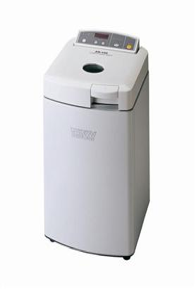
\includegraphics[width=.3\textwidth]{img/centrifugal.png}\hfill
            % \includegraphics[width=.3\textwidth]{img/vacuum.jpg}\hfill
            \caption{Centrifugal Mixer}
            % \caption{Vacuum for Degassing}
        \end{figure*}
    \end{multicols}
\subsection{Mold Making Process}
\begin{enumerate}
    \item Grab your paper cup and cut it until it fits the centrifugal bottle holder
    \item Put your paper cup on the scale and start pouring silicone solution
    \item The manufacture of your silicone solution have weight ratio, use that to create your solution (eg, Smooth sil uses 10:1 ratio of product A and B). Use popsicle sticks to accurately get the mass you need 
    \item Once you are done, measure the weight of the whole bottle with your polymer solution (bottle holder, solution, bottle cap), take a note of this
    \item Insert the bottle holder to the centrifugal mixer, there is only one correct way to align it and the centrigufal mixer will help you orienting it.
    \item Adjust the weight by scrolling the knob inside the centrifugal mixer to match the weight of the whole bottle holder
    \item Change memory to 1 if not done yet. Memory 1 have 30s of mixing and 30s of defoaming
    \item press start, and wait until it finish
    \item Once the defoaming process is done, it will beep. Take out the bottle and your mixed solution
    \item Check your solution, if it is mixed continue; else mix it again. Beware that mixing it for too long will produce heat which will make your mold too stiff (see \href{Mold_Tables}{Appendix})
    \item Vacuum your solution until the rate of bubble formation is slow\\
        \begin{centering}
        $%\Teaser{
    \TeaserImage{img/Vacuum_1.jpg}
    \Rightarrow
    \TeaserImage{img/Vacuum_2.jpg}
    \Rightarrow
    \TeaserImage{img/Vacuum_3.jpg}
    $
\end{centering}
    \item While you wait for vacuum to finish, it is a good time to spray your mold with the non-stick spray, do this under the fume hood.
    \item Once vacuum is done, take it out of the vacuum pump
    \item Fill your mold with the polymer solution
    \item Let it cure for a whole day (you can use oven to speed up the process if you want, some polymer can only cure in high temperature as well, again see manufacture data sheet to be sure)
    \item Clean up and tidy everything
    \item Once it's cured, take it out of the mold
\end{enumerate}
\section{Safety}
\section{Appendix}
\subsection{Mold Tables Important Property}\label{Mold_Tables}
\subsection{Contact Information}

\end{document}
